\section{Products and service table}\label{sec:service}
MPX offers four products: \emph{transfers} between home ledgers; \emph{spot} in lots of $1{,}000$ units, tick $0.01$ credits; \emph{futures} with TDB expiries, cash-settled at the expiry batch price; and a \emph{delivery guarantee} paying face value if a transfer's endpoint attempt is abandoned, at a fair premium equal to that probability. Spot and futures require margin (R6) and member liquidity of $30\%$ of notional. Clearing fees, the operators' $0.10\%$ band fee and the guarantee loading fund MPX's operating capital.
\begin{table}[H]
\centering
\caption{Service at hour 0 by settlement ($\sigma=30\%$). Transfer times are to the Earth hub: credit after one way, final after the confirmation returns.}\label{tab:service}
\small
\begin{tabular}{@{}lp{0.13\linewidth}lp{0.1\linewidth}lp{0.11\linewidth}p{0.2\linewidth}@{}}
\toprule
Settlement & Access, batch & Copies & Credit / final (h) & Margin & Guarantee premium & Restrictions \\
\midrule
Mercury & member, fast & 3--4 & 0.77 / 1.53 & 1.93\% & $2.0\times10^{-5}$ & send up to 76 min early \\
Venus & member, fast & 3--4 & 0.68 / 1.35 & 1.94\% & $1.1\times10^{-5}$ & \\
Earth & hub, fast & 1 & local & 1.33\% & 0 & \\
Mars & member, fast & 2--4 & 0.57 / 1.13 & 1.95\% & $5.4\times10^{-6}$ & \\
Ceres & member, fast & 2--4 & 0.56 / 1.11 & 1.98\% & $5.2\times10^{-6}$ & B link closed h 240--264 \\
Jupiter & member, fast & 3--4 & 0.85 / 1.70 & 2.09\% & $2.9\times10^{-5}$ & \\
Saturn & member, full & 3--5 & 1.32 / 2.65 & 2.27\% & $3.4\times10^{-4}$ & orders every 6 h only \\
Uranus & operator, full + local & 5--7 & 2.64 / 5.28 & 2.67\% & $6.6\times10^{-3}$ & local quotes within $\pm1.46\%$ \\
Neptune & operator, full + local & 7--9 & 4.17 / 8.35 & 3.01\% & $3.3\times10^{-2}$ & local quotes within $\pm1.82\%$; B closed h 2--26 \\
\bottomrule
\end{tabular}
\end{table}
\vspace{-6pt}
\section{Responsibilities when messages fail}\label{sec:fail}
Authority is fixed: the hub decides batches, fills and margin; the destination ledger decides whether a transfer was credited; the source ledger decides debits. No actor ever infers another's decision from silence.
\begin{table}[H]
\centering
\caption{What each actor knows, does and owes.}\label{tab:fail}
\small
\begin{tabular}{@{}p{0.13\linewidth}p{0.26\linewidth}p{0.26\linewidth}p{0.26\linewidth}@{}}
\toprule
Failure & Order (sender, hub) & Transfer (source, destination) & Margin call (hub, member) \\
\midrule
Lost & Hub knows nothing. Sender learns from the accepted-ID broadcast, owes nothing, may resubmit next batch & Hop retries, then endpoint attempts. Source knows only ``pending'', keeps the hold. Destination owes nothing until a copy arrives & Hub knows the call is unanswered at its deadline and resends once. Member owes the top-up from when it receives the call \\
Late & Rejected late (R4); listed as rejected. Sender's position unchanged & Valid until $E$ unless cancelled. After $E$ or a CANCEL, the destination tombstones it and signs NOT-CREDITED; the source refunds & A payment after the deadline still counts; default only after the resend round expires \\
Duplicated & First valid copy filled; others receipted and ignored. At most one fill per ID & First copy credited; later copies receipted, never credited twice & Repeat calls with the same ID ask for the same top-up once \\
Contradicted & Same ID, different content: both rejected, sender flagged; hub's record of fills is final & Destination's signed CREDITED or NOT-CREDITED is final; it can sign only one & Hub's statement prevails; disputes settle at the next batch statement \\
\bottomrule
\end{tabular}
\end{table}
\vspace{-6pt}
\begin{table}[H]
\centering
\caption{Order lifecycle. Each state has exactly one authority; no state is inferred from silence.}\label{tab:life}
\small
\begin{tabular}{@{}lp{0.12\linewidth}p{0.33\linewidth}p{0.3\linewidth}@{}}
\toprule
State & Authority & Entered when & Leaves to \\
\midrule
Created & sender & client submits; ID assigned & Sent \\
Sent & sender & $k$ copies launched by $T_b-(\ell-\lfl)-60\,$s & Valid or Rejected late \\
Valid & hub & first copy arrives by $D_k$ & Cleared \\
Rejected late & hub & no copy by $D_k$; listed in the accepted-ID broadcast & terminal; may resubmit \\
Cleared & hub & batch clears at $T_b+\max\lfl$ & Filled or Unfilled \\
Filled / Unfilled & hub & uniform-price match decided & Reported \\
Reported & hub & fill report sent; position and margin updated at the hub & Confirmed \\
Confirmed & sender & report received; sender's view matches the hub & terminal \\
\bottomrule
\end{tabular}
\end{table}
\vspace{-6pt}
\section{Assumptions}\label{sec:assume}
\begin{table}[H]
\centering
\caption{Assumptions, kept apart from proofs and limits.}\label{tab:assume}
\small
\begin{tabular}{@{}lp{0.56\linewidth}p{0.3\linewidth}@{}}
\toprule
\# & Assumption & Used by \\
\midrule
A1 & The brief's frozen ellipses, constants, loss model, quotas and maintenance are exact & everything \\
A2 & Launches are lost independently, as the brief states & copies, E2 \\
A3 & Price returns: $\sigma=30\%$ a year; Student-$t_3$ tails for margin & R6, E5 \\
A4 & Messages are signed; keys identify the origin settlement & G3, G4 \\
A5 & Members hold liquid resources of $30\%$ of notional, recertified monthly & R6, E5 \\
A6 & Batch, transfer and statement messages fit one packet each & quota counts \\
A7 & Deterministic S1 price paths of $\pm0.5\%$ per fast batch; the S2 incident is our choice & S1, S2 \\
A8 & Direct service is used only for incident notices, within its 12-copy daily allowance & E2 \\
\bottomrule
\end{tabular}
\end{table}
\vspace{-6pt}
\section{Guarantees and their conditions}\label{sec:guar}
\textbf{G1 Connectivity} (Sun only). Relays A and B share a $\sqrt8\AU$ circle, $90^\circ$ apart, so their chord passes the Sun at $2\AU$. For a settlement at radius $r$, a blocked relay lies within $\arcsin(0.1(1/r+1/\sqrt8))\le21.13^\circ$ of its antipode (worst case: Mercury at perihelion), so the two relays are never blocked together. \emph{Proof.} A closure needs the segment's nearest point to the Sun inside it (both endpoints lie at least $0.3075\AU$ out). Then the angle $\theta$ at the Sun between the settlement $P$ and the relay $R$ satisfies $\sin(\pi-\theta)\cdot r\sqrt8 = 2\cdot\text{area} = |P-R|\cdot\text{dist} \le |P-R|\,0.1 \le (r+\sqrt8)\,0.1$, giving the bound. The relays are $90^\circ$ apart and each blocked cone is at most $2\times21.13^\circ$ wide, so no direction blocks both. Projecting to the ecliptic only shortens distances, so the planar case covers 3D. $\square$ \emph{Condition:} no maintenance or incident on both a settlement's relay links.

\textbf{G2 No closure missed.} Clearance is $V$-Lipschitz with $V=\max(v_s, v_r(1+2\vmax/(c-\vmax)))$ (perihelion speeds), so an hourly sample below $0.10+V/2$ flags every closure; flagged hours are refined to 1 minute and boundaries bisected to $10^{-7}\h$.

\begin{figure}[H]
\centering
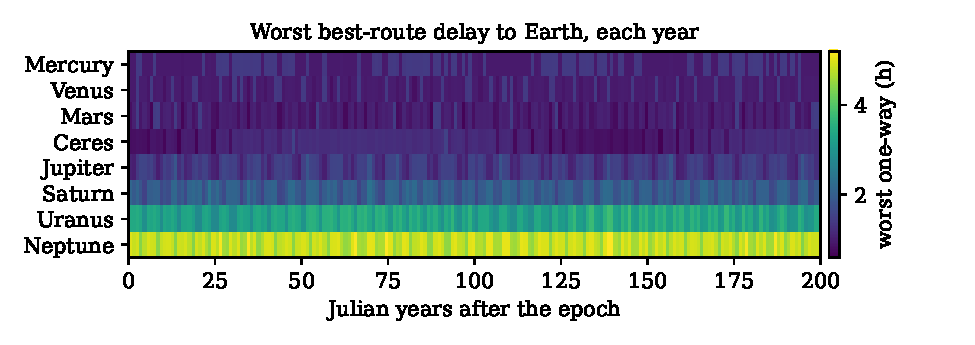
\includegraphics[width=\linewidth]{fig_heatmap.pdf}
\vspace{-14pt}
\caption{E4 at a glance: the worst best-route delay to Earth in each of 200 years. Every cell is finite (G1); Neptune never exceeds $5.19\h$.}
\end{figure}
\vspace{-6pt}
\textbf{G3 Causal fairness (Light-Cone Clearing).} An order arriving by $T_b+\lfl$ left its origin by $T_b$, since no path beats the straight line, including the faster direct service. \emph{Condition:} the hub knows each order's origin (signed keys).

\textbf{G4 Exactly-once transfers and conservation.} The destination signs at most one of CREDITED or NOT-CREDITED per ID: it credits only an ID it has not tombstoned, and it tombstones (signing NOT-CREDITED) only an ID it has not credited; both decisions are local to one single-writer ledger, so they cannot both occur. The source moves the hold exactly once, on that signature. At every instant each unit of value is in exactly one place: available, held at the source, in flight, or credited at the destination. Total funding is constant, and no unit is spendable in two places. \emph{Proof.} Every ledger action is a double entry summing to zero, so total funding is invariant. Transfer $T$ has three phases: before credit (value in flight, source holds a non-spendable memo), credited (spendable only at the destination), refunded (spendable only at the source). Credit and tombstone are mutually exclusive decisions of one single-writer ledger. The source moves only on the destination's signed decision. Hence $T$ ends credited or refunded, never both, and no phase makes the value spendable in two places. Retries and copies carry the same ID, so they can trigger at most one credit. $\square$ (E3 checks this in every scenario.)

\textbf{G5 At most one fill per order}, by ID deduplication (R3); copies can never multiply a position.

\textbf{G6 On-time deadline messages}: probability at least $99.5\%$, from $f$ at send time. \emph{Condition:} independent launches, which incidents break (handled by R8, not by probability).

\textbf{G7 Margin coverage.} IM covers $99\%$ of price moves over the MPOR for Student-$t_3$ returns; Gaussian returns exceed it only $0.45\%$ of the time (E5). \emph{Condition:} the call is delivered. A call or answer misses its first window with probability at most $1-0.995^2=1.0\%$; the resend then stretches Neptune's window from $12.9$ to $23.3\h$, where $t_3$ exceedance is $2.16\%$. The total is $0.99\times1.0016\%+0.01\times2.16\%=1.013\%$.

\textbf{G9 Swap atomicity.} A hash-locked swap ends with both legs done or both refunded. \emph{Proof.} The seller can claim only with the secret, which the buyer reveals only by claiming the asset; once revealed, the secret reaches the buyer's ledger within one light-time, and the buyer's lock outlasts that. If the buyer never claims, both locks expire and each side refunds. $\square$ \emph{Condition:} locks set as in R8b.

\textbf{G10 One hub at a time.} If Mars last received a renewal sent at time $r$, Earth's lease ended by $r+4\h$, while Mars waits until at least $r+5\h$. Earth counts only renewals Mars has acknowledged, so its view is never later than Mars's. Their clearing intervals cannot overlap. $\square$ \emph{Condition:} both hubs keep TDB time (R1 clocks).

\textbf{G8 Finality bound.} No ledger can confirm a spend faster than light can reach another replica that could approve a conflicting one; single-writer home ledgers satisfy this by design \cite{gilbert2002}.

\section{Risks and limits}\label{sec:risk}
\begin{table}[H]
\centering
\caption{Ranked risks: severity and likelihood from 1 to 3, rank by their product, ties broken by severity.}\label{tab:risk}
\small
\begin{tabular}{@{}rp{0.18\linewidth}ccp{0.27\linewidth}p{0.27\linewidth}@{}}
\toprule
\# & Risk & Sev & Lik & Evidence & Control \\
\midrule
1 & Trend exhausts member liquidity & 3 & 2 & 15\% trend, 10\% jump and isolation: $18.45\%$ of rising runs default (E5) & 30\% liquidity rule; Cover-2 fund at 6\,sd; recovery used in 0.03--0.05\% of runs \\
2 & Outer member isolated (incident on top of maintenance) & 3 & 2 & Relay A loss h 0--6 with B--Neptune maintenance isolates Neptune (S2) & Notice by direct service; re-pin; hedge, not default (R8) \\
3 & Queue overflow on a pinned route & 3 & 1 & Cap fills in $16.7$ days; closures last up to $190$ days & Re-pin before every predicted closure (R1) \\
4 & Lost margin call & 2 & 2 & $0.2$--$0.4\%$ of calls miss on first send (E5) & Copies; one resend round before default (R6) \\
5 & Fat-tailed prices & 2 & 2 & Gaussian multiplier breached $1.38\%$ (E5) & Multiplier 2.62; 6\,sd fund stress \\
6 & Quota crunch on incident days & 2 & 1 & Worst day 468 for batches; calls peak at 56 a day & 132 originations reserved; adaptive copies \\
7 & Model error vs real ephemeris & 1 & 3 & Earth drifts up to about 4{,}700 km, $15.6$\,ms (\cref{sec:effects}) & 60 s send-early margin \\
8 & Duplicates and conflicts & 3 & 1 & Copies, retries and receipts all create duplicates & ID deduplication; authority table (\cref{tab:fail}) \\
9 & Hub outage at Earth & 3 & 1 & Earth is a single clearing point & Mars standby with leases; no overlap (R8f, G10) \\
10 & Quota exhausted mid-incident & 2 & 1 & Calls, re-pins and orders compete & Fixed priority order (R8e) \\
\bottomrule
\end{tabular}
\end{table}
\begin{figure}[H]
\centering
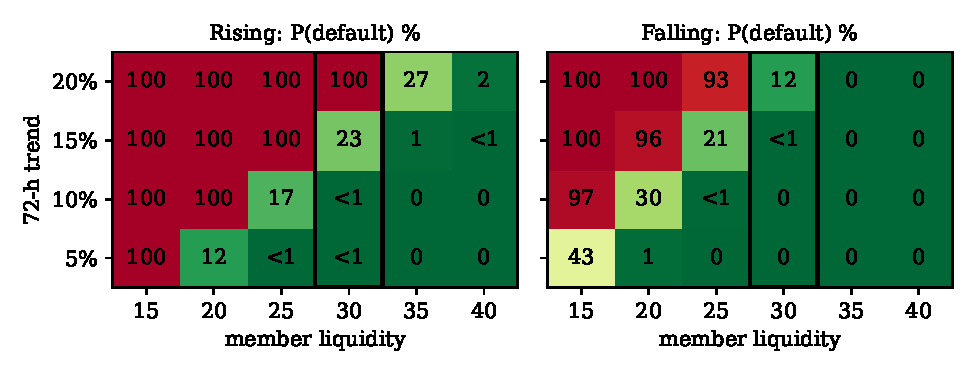
\includegraphics[width=\linewidth]{fig_phase.pdf}
\vspace{-14pt}
\caption{Failure boundary (E5 Tier 3, 600 runs per cell): probability of a member default against member liquidity and the 72-hour trend, with a 10\% jump, fat tails and a Neptune isolation on top. The boxed column is the design's 30\% rule; defaults appear only when the trend outruns liquidity, in either direction.}
\end{figure}
\vspace{-6pt}
\textbf{Interactions.} (i) More copies raise on-time delivery but spend quota: adaptive copies cut the worst day from 496 to 468 originations. (ii) Straight-line deadlines make batches fair but cost Mercury up to 76 minutes of information. (iii) An isolation plus a falling price stresses margin while calls cannot be delivered: R8 caps exposure at the MPOR. (iv) Maintenance turns a 6-hour relay incident into a full Neptune isolation that would otherwise cost 45 minutes (S2). (v) The liquidity rule protects the waterfall but ties up $30\%$ of notional: capital efficiency trades against default risk (E5 sensitivity).

\textbf{Limits.} Batches clear at most every $1.5\h$; Saturn, Uranus and Neptune trade every $6\h$; positions need liquidity of $30\%$ of notional; a refund needs the destination's signature, one round trip after CANCEL (up to $10.4\h$ for Neptune).
